\chapter{Technical Work}
\label{ch:tw}

%In this chapter we will discuss the experiments and the process that has been followed to develop the model for predicting the amplifier output profile


\section{Introduction} 
\label{tw:intro}

This chapter will discuss the experiments that have been carried out and the process that has been followed, leading to the development of a machine learning model capable of predicting the output power spectrum of an EDFA. 
The work that has been undertaken will be split into sections as follows:
\begin{enumerate}
    \item Amplifier characterisation, a detailing of the experiments carried out to characterise the amplifier model that has been used throughout this thesis.
    
    \item Data generation will discuss the experiment that has been designed to generate suitable training data facilitating the development of the machine learning model.
    
    \item Model Design will outline the development of the baseline machine learning model, the development environment and the design choices made during the development process.
    
    \item Sensitivity Analysis will discuss the analysis of the model from section \ref{sec:ml_model}. This analysis aims to determine a strategy for reducing the amount of training data required by the ML model.
    
    \item Pruning and Quantisation will discuss the optimisation methods that have been applied to improve the model in terms of memory requirements, training time and model complexity. 
\end{enumerate}



%%%%%%%%%%%%%%%%%%%%%%%%%%%%%%%%%%
% Beginning of New Section Here
%%%%%%%%%%%%%%%%%%%%%%%%%%%%%%%%%%

\newpage
\section{Amplifier Characterisation}
\label{tw:sec:amp_char}


\subsection{Introduction}
This section will detail the characterisation experiment carried out on the amplifier model used throughout this project. In place of a physical EDFA amplifier, a virtual model from a photonics simulation software package was used. The following section will also provide a detailed description of the software package used.

The need to carry out an experimental characterisation of the EDFA arises from the necessity to verify the accuracy of the virtual model to one of a physical amplifier. This process will determine characteristics of the amplifier, such as the gain profile, the impact of noise on the amplifier output and the amplifier fidelity, in terms of the presence of saturation effects and interaction effects between the various input channels. This characterisation will inform the design of later experiments and the development of the machine learning model itself.

\subsection{Amplifier model}
An EDFA model from the VPI Photonics software package (VPI) was used for this experiment. VPI is a photonics design tool specifically suited to the modelling of fibre optics and optical amplifiers. There are a variety of amplifier models available from the VPI software. 

A black box amplifier, “AmpBlackBoxOpt”, was used throughout this project. It is a model of an EDFA amplifier based on data measured from a physical device. The amplifier output accounts for wavelength-dependent gain and noise spectra. The amplifier operation can be controlled by a set gain value, a set output power value, or can operate in constant saturation mode.

This experiment will characterise the amplifier model; this is necessary to verify that the amplifier will operate as expected under a simulated network traffic load.  The experiment should:

\begin{itemize}    
    \item Determine the output gain profile; this will show whether a gain flattening filter has been applied to the amplifier output.\\

    \item Determine if the amplifier model has a saturation point, and if so what it is.\\
    
    \item Verify that the amplifier model accounts for interaction effects between input channels.\\
\end{itemize}





\subsection{Experimental Setup}
The experimental setup to characterise the amplifier is shown in figure \ref{fig:tw_amp_char}.
The amplifier input consists of 3 optical signal sources multiplexed together:

\begin{figure}
    \centering
    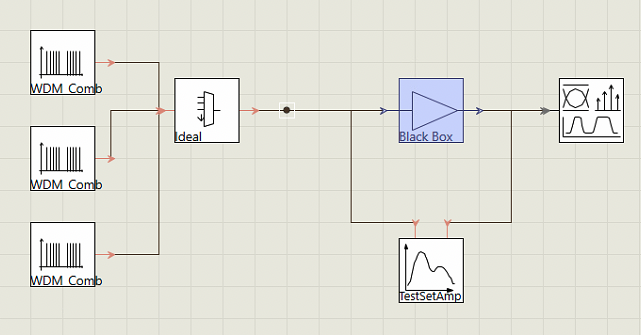
\includegraphics[width=\linewidth]{images/technical_work/section_1_characterisation/amp_char_ex_setup.png}
    \caption{Experimental Setup in VPI}
    \label{fig:tw_amp_char}
\end{figure}


\begin{enumerate}
    \item The primary input source, generated by a WDM comb module outputting 44 channels spaced in 100GHz intervals, over the range: 192.THz - 196.3THz. This frequency range and spacing were chosen as it adhered to the frequency spacing of the ITU DWDM frequency grid. The output channel power was set at 50$\mu$W as to emulate a realistic input to an EDFA that might occur in an actual network scenario. \\
    
    \item The lower variable source, this optical source will output a single channel at a frequency of 192.5. The output power of the signal will be varied during the experiment.\\
    
    \item The upper variable source will mirror the lower variable source at a frequency of 195.8; its output power will also be varied during the experiment.  
\end{enumerate}


The three signal sources are combined using an ideal multiplexer and inputted to the black box amplifier. The output of the amplifier was sent to an optical signal analyser to be graphed.

The output powers of the lower and upper sources were varied from a value of 1$\mu$W to 1W in 5 steps. Only one optical signal from either source was active during a given step.



\subsection{Results}

The results of the experiment can be seen in figures \ref{fig:tw_amp_char_lc} and \ref{fig:tw_amp_char_uc} , where the output spectrum as a result of varying the lower source is shown in figure \ref{fig:tw_amp_char_lc} and as a result of varying the upper source is shown in figure \ref{fig:tw_amp_char_uc}. 

The interaction effects between channels can be seen by examining the change in the output spectrum as the two sources are varied. The higher frequency channel has a much more significant impact on the overall output spectrum than the lower frequency channel of the same power. The gain of the entire output spectrum is suppressed as the power of the high-frequency channel is increased. In contrast, increasing the power of the lower frequency channel results in a marginal increase in the power of output spectrum. 


\renewcommand{\arraystretch}{0.5}
\begin{figure}
    \floatpagestyle{empty}
    \centering
    \caption{Shows the effect the power of the lower channel has on the gain spectrum.}
    \begin{tabular}{c}
        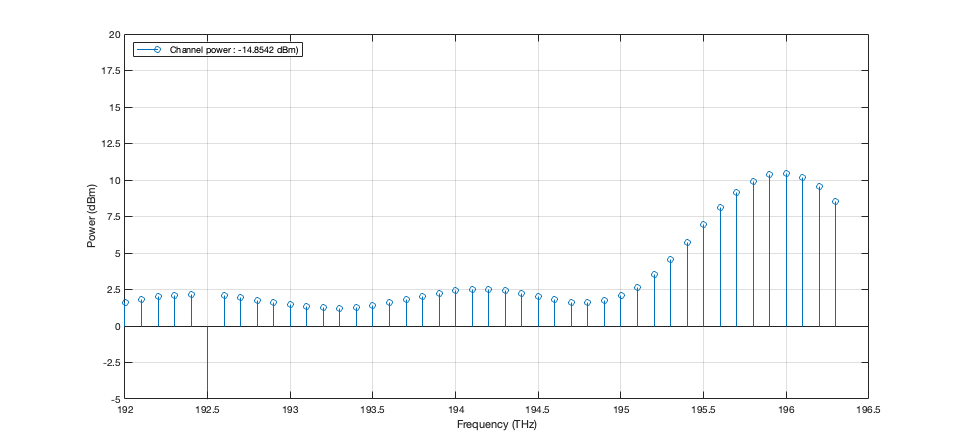
\includegraphics[width=0.85\textwidth]{images/technical_work/section_1_characterisation/figures/1.png} \\
        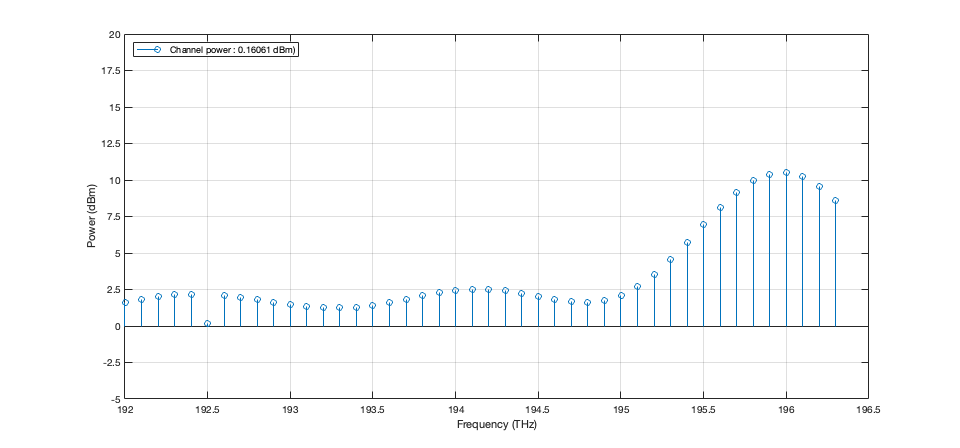
\includegraphics[width=0.85\textwidth]{images/technical_work/section_1_characterisation/figures/2.png} \\
        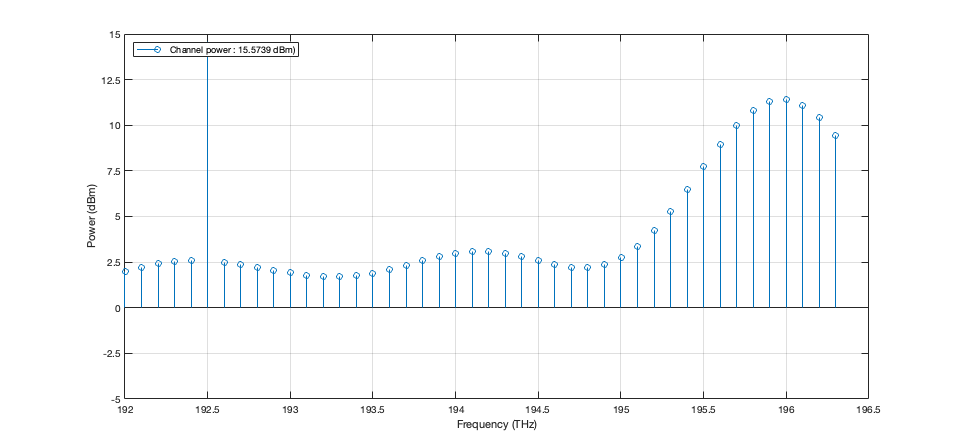
\includegraphics[width=0.85\textwidth]{images/technical_work/section_1_characterisation/figures/3.png} \\
        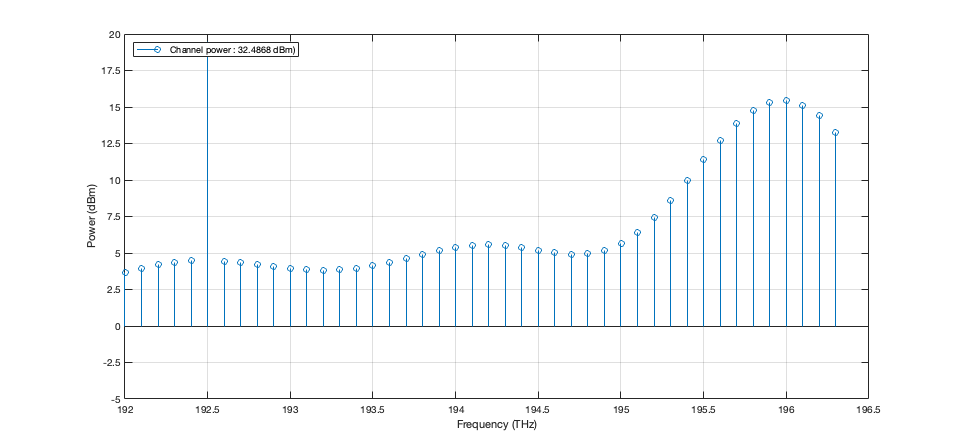
\includegraphics[width=0.85\textwidth]{images/technical_work/section_1_characterisation/figures/4.png} \\
    \end{tabular}
    \label{fig:tw_amp_char_lc}
\end{figure}

\begin{figure}
    \floatpagestyle{empty}
    \caption{Shows the effect the power of the upper channel has on the gain spectrum.}
    \centering
    \begin{tabular}{c}
        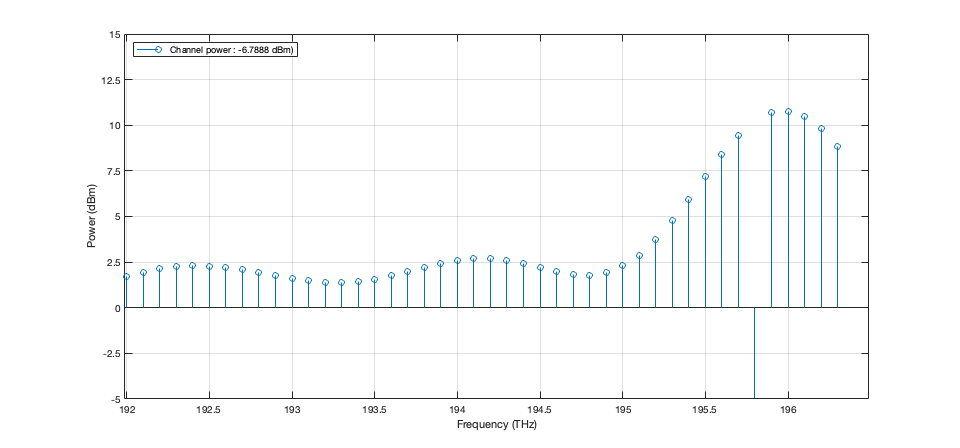
\includegraphics[width=0.85\linewidth]{images/technical_work/section_1_characterisation/figures/6.png} \\
        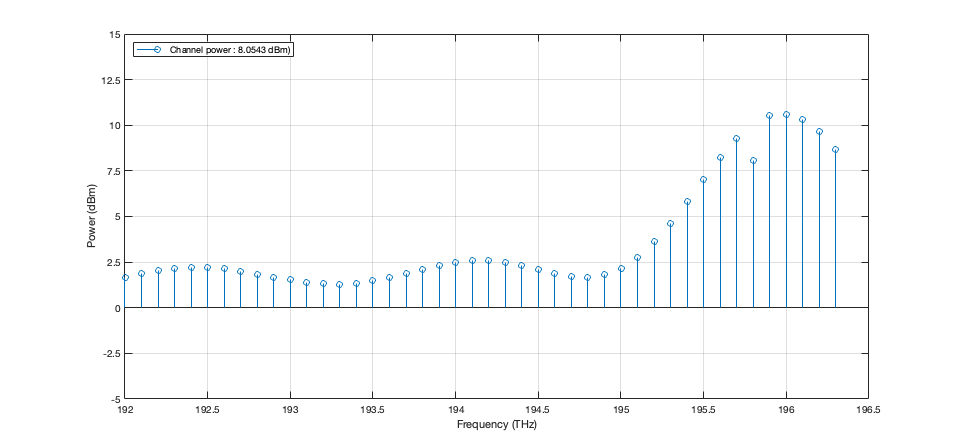
\includegraphics[width=0.85\linewidth]{images/technical_work/section_1_characterisation/figures/7.png} \\
        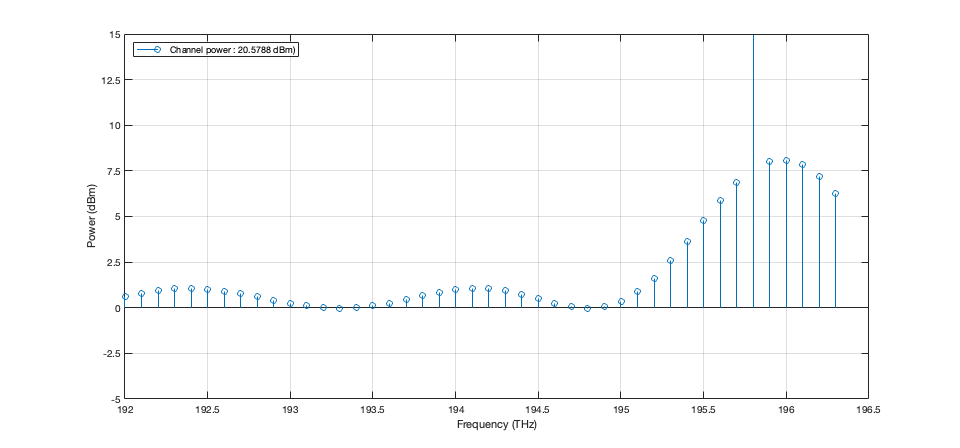
\includegraphics[width=0.85\linewidth]{images/technical_work/section_1_characterisation/figures/8.png} \\
        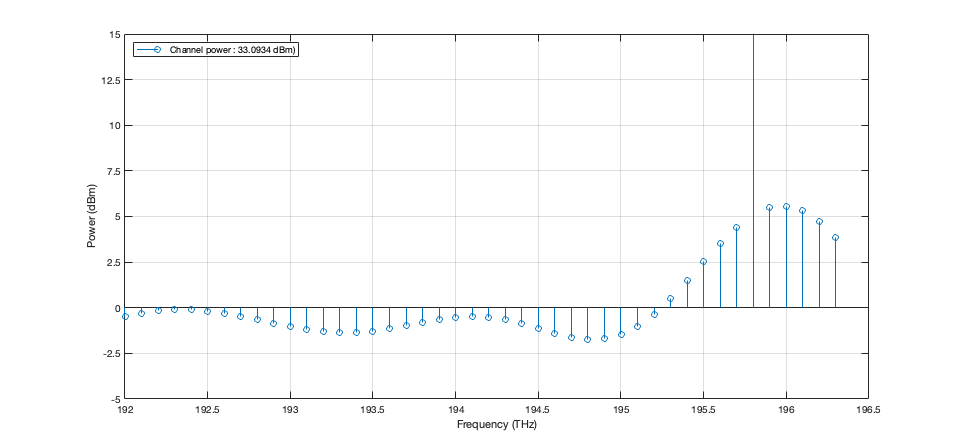
\includegraphics[width=0.85\linewidth]{images/technical_work/section_1_characterisation/figures/9.png} \\
    \end{tabular}
    \label{fig:tw_amp_char_uc}
\end{figure}


\subsection{Conclusion}
From the experimental results in figures \ref{fig:tw_amp_char_lc} and \ref{fig:tw_amp_char_uc} it can be clearly seen that the amplifier does not have a gain flattening filter applied as its output spectrum is non-flat. The amplifier model does not have a saturation point; the gain of the two variable channels did not reduce as their powers increased. The model accounts for interaction effects between channels, as evidenced by the alteration of the output spectrum when the power of the variable sources is increased.

This experiment served as a means to characterise the amplifier by studying the impact of one channel on the entire output spectrum. This project aims to analyse and predict the impact that all other channels have on a single channel. Predicting the impact on a single channel will be the subject of experiments in subsequent sections; the results from this experiment will be used to inform the design of these experiments.


%%%%%%%%%%%%%%%%%%%%%%%%%%%%%%%%%%
% Beginning of New Section Here
%%%%%%%%%%%%%%%%%%%%%%%%%%%%%%%%%%


\FloatBarrier
\section{Data Generation Experiment} \label{tw:sec:data_gen}


\subsection{Introduction}

This section will discuss the experiment used to generate training data for the ML model. The training data must emulate optical signal traffic from real-world scenarios to provide the model with suitable data to predict the output spectrum amplifiers used in optical networks.


\subsubsection{Experiment Parameters}

The ITU define a frequency grid for DWDM applications centred at 193.1THz and using channel spacings up to 100GHz. The frequency range from 1530nm (195.943THz) to 1565nm (191.561THz), known as the C band in fibre optic communications. The C band is the primary wavelength used for long-distance optical communication, as it is in this frequency band where fibre optic cables have the lowest losses. 

The channel spacing was set at 100GHz to conform to the standard ITU DWDM frequency grid. A common channel plan found in many DWDM systems is to use 44 channels spaced at 100GHz or 88 channels spaced at 50GHz. In this case, 44 channels spaced in 100GHz intervals from 191.6THz to 195.9THz will be used.  

The channel power was set at $50\mu W$, as this reflects a typical channel input power for an EDFA in an optical communications network. The input power was not varied between channels.

Maintaining a constant channel power has several implications for the model that will be trained on this data. As a result of applying this restriction, the model will not account for cases where the power of all channels is varied from $50\mu W$ or where the channel powers are not uniform. 

This restriction will reduce variability in the training data and enable the model to learn the effects of different channel loading conditions more easily. The impact that channels have on each other will be solely due to their relative frequency, as opposed to their relative power and relative frequency.


Each training data sample will consist of two arrays, both 44 units long. The VPI simulator randomly generates the array of input powers, and the corresponding array of output powers is measured from the amplifier’s output. The training samples can vary in the following ways:
\begin{itemize}
    \item The input power of each of the 44 channels will either be 0W or $50\mu W$. The number and location of the non-zero channels will be randomly set.
    
    \item The output powers will either be $0\mu W$ if the input power of that channel was $0\mu W$ or will be some non-zero value of power determined by the channel-specific gain.
\end{itemize}

The gain of each channel will depend on the channel loading conditions, i.e., the relation between the frequency of a particular channel and all other “on” channels.



\subsection{Experimental Setup}
\FloatBarrier

\begin{figure}[h]
    \caption{Experimental setup in VPI. Figure \ref{fig:tw:top_lvl} shows the top level simulation. Figure \ref{fig:tw:co_sim_galaxy} shows the expanded co-simulation sub-module, referred to as a galaxy.}
    \begin{subfigure}{\textwidth}
        \centering
        \caption{From left to right, the co-simulation galaxy, EDFA amplifier and the optical systems analyser.}
        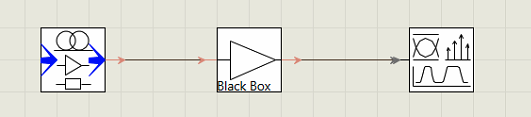
\includegraphics[width=0.8\textwidth]{images/technical_work/section_2_data generation/ex_setup.png}
        \label{fig:tw:top_lvl}
    \end{subfigure}
    \begin{subfigure}{\textwidth}
        \centering
        \caption{Expanded co-simulation galaxy, showing the co-simulation model being used as an output.}
        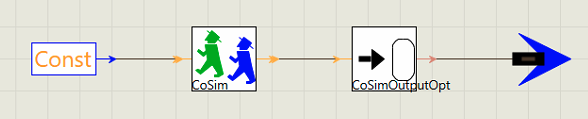
\includegraphics[width=0.8\textwidth]{images/technical_work/section_2_data generation/co_sim_galaxy.png} 
        \label{fig:tw:co_sim_galaxy}
    \end{subfigure}
    \label{fig:tw:exp_setup}
\end{figure}


The experimental setup to generate the training data is shown in figure \ref{fig:tw:exp_setup}. The experiment will generate a random channel loading scenario. A random number of channels $n$, between 2 and 44 inclusive, will be turned “on” i.e., have an input power of $50\mu W$. The frequency of each “on” channel will also be randomly decided. 

The scenario where the input is a single channel will be ignored. As in this case, the single-channel will not be impacted by any other channels.

The $n$ channels will be inputted to the amplifier. The value of the corresponding $n$ output channels along with the $n$ input channels will be recorded. This process will be repeated several thousand times to generate sufficient data to train the ML model. 

As in the experiment from section \ref{tw:sec:amp_char}, the amplifier model from VPI will be used. However, there is no straightforward method to generate a random array of channels in VPI. The array of input channels will be generated using MATLAB and then be read into VPI using the simulators co-simulation function.

As seen in figure \ref{fig:tw:exp_setup} the experimental setup consists of setting the output of the MATLAB co-simulation module as the input to the optical amplifier and measuring the output of the optical amplifier using the optical systems analyser module. 


\subsubsection{MATLAB Channel Generation} \FloatBarrier

Though the optical channels are generated in MATLAB, for them to be read by VPI, they must conform to the internal structure that VPI has defined for optical signals. 

Optical signals in VPI are comprised of noise bins, sampled bands, and parameterised signals; all three signal components must be created for a signal to be used in VPI. 
In this experiment, we are only interested in the parameterised signals.

Cell arrays represent the VPI optical signal components in MATLAB. Thus a cell array for each component will be created. Only the parameterised signal cell array will contain the values of our channels.  

The MATLAB code used to generate the channels can be found in appendix \ref{}.

Each time a training sample is generated, the MATLAB script is run. Before a sample is generated, the random number generator used to select the channels is re-initialised using the current time, ensuring the channel loading conditions are indeed random and independent from each other. 


\subsubsection{Verification}

\begin{figure}[h]
    \centering
    \caption{Results of 5000 dummy runs of the channel generator.}
    \label{fig:tw:dummy_runs}
    \begin{subfigure}{0.49\textwidth}
        \centering
    \caption{Plot of the relative occurrence of each channel.}
    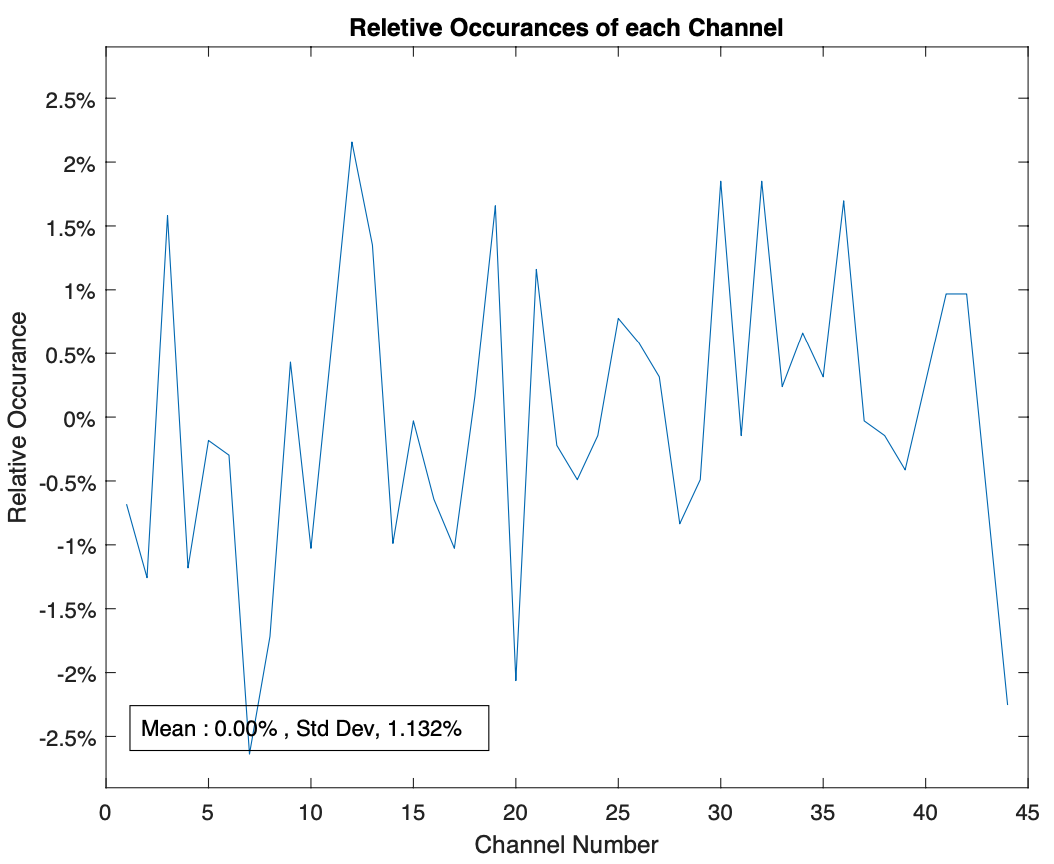
\includegraphics[width=\textwidth]{images/technical_work/section_2_data generation/rel_occur_ch.png}
    \label{fig:tw:data_gen:rel_ch}    
    \end{subfigure}
    \begin{subfigure}{0.49\textwidth}
        \centering
        \caption{Plot of the relative occurrence of the number of channels generated, note the y-axis i scaled by $1e^{-3}$.}
        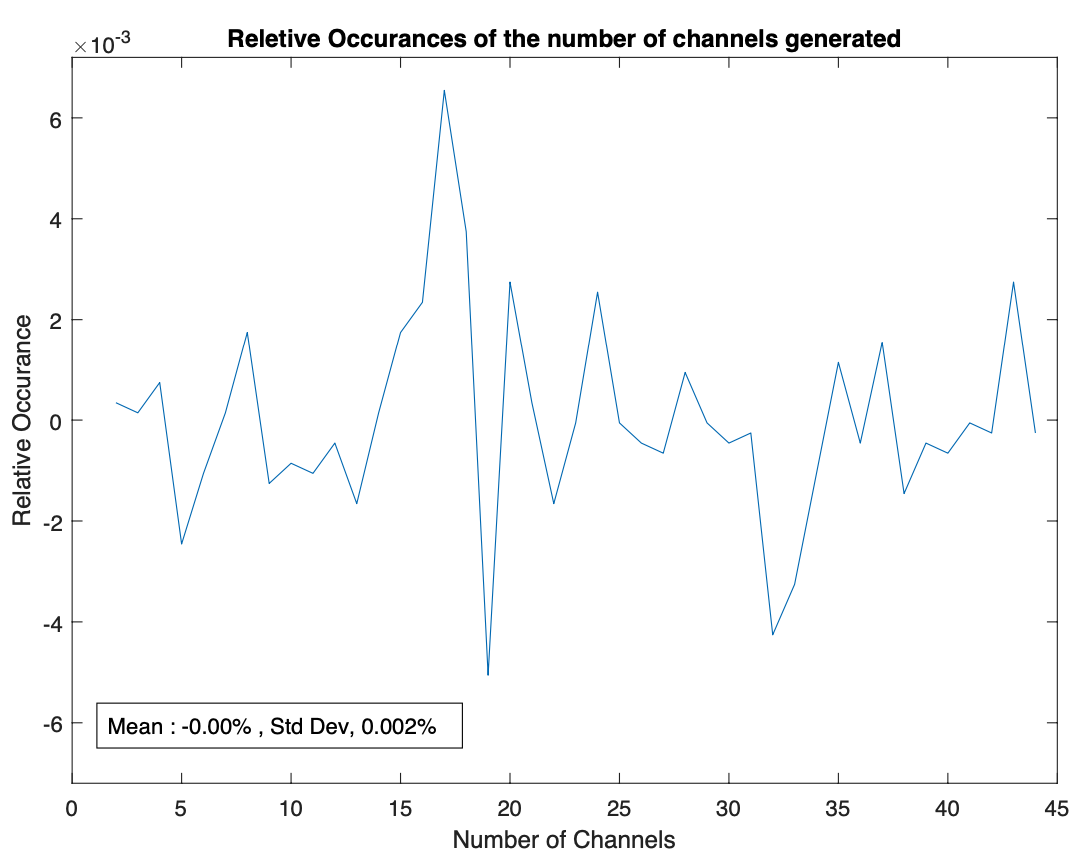
\includegraphics[width=\textwidth]{images/technical_work/section_2_data generation/rel_occur_num_ch.png}
        \label{fig:tw:data_gen:rel_num_ch}
    \end{subfigure}
\end{figure}


A verification script was created to ensure that the channel generation scrip was functioning as expected.

The verification script records the output of the channel generator over a number of runs and plots the results. The results of performing 5000 runs can be seen in figures \ref{fig:tw:data_gen:rel_ch} and \ref{fig:tw:data_gen:rel_num_ch}. 

As can be seen from the figures, there is no bias towards any particular channel nor a particular number of channels. The variation in the relative occurrence of the channels and the number of channels generated can be attributed to the number of dummy runs produced and expected to decrease where the number of runs increased. Ensuring that there are no biases in the underlying data used to train the model is critical. Further discussion on this can be found in section \ref{}. The script used to verify the channel generator can be found in appendix \ref{}.

\FloatBarrier

\subsection{Results}

A selection of training data samples generated by the simulator can be seen in figure \ref{fig:tw:vpi_samp_op}. In figure \ref{fig:tw:vpi_50_op} the variation in the outputs of the channels can be seen. The variation results from the impact that different channel loading conditions have on the amplification of each channel.

\begin{figure}[!h]
    \centering
    \caption{Sample outputs from the VPI simulator.}
    \label{fig:tw:vpi_samp_op}
    \begin{subfigure}{\textwidth}
        \centering
        \caption{One sample run from the simulation.}
        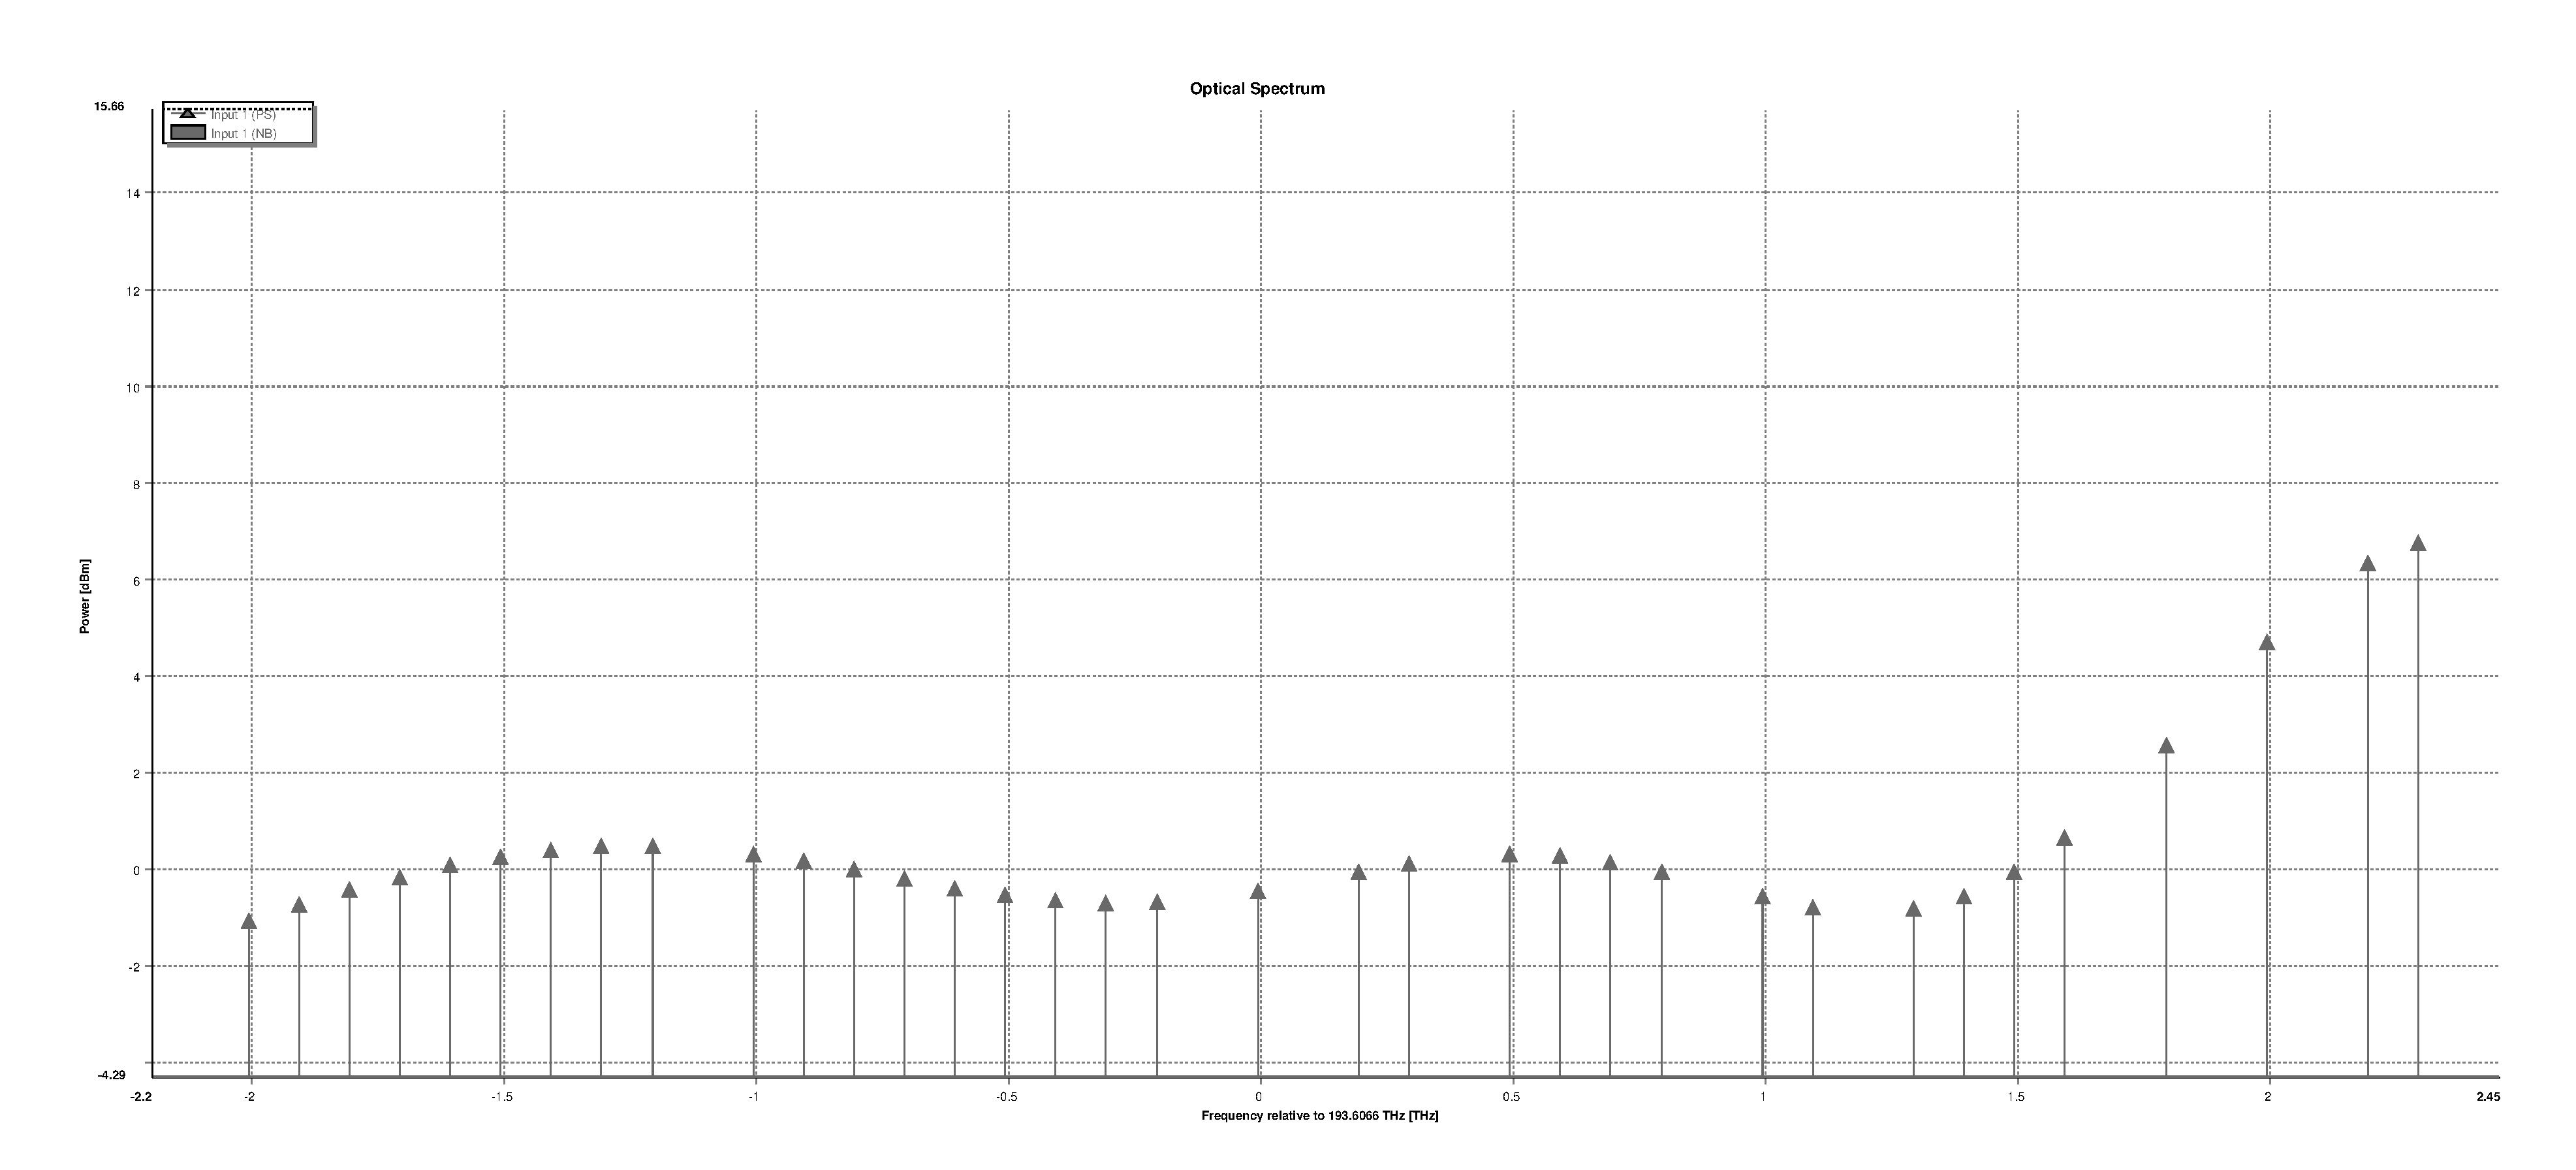
\includegraphics[width=\textwidth]{images/technical_work/section_2_data generation/sample_output_1.pdf}
        
        \label{fig:tw:vpi_1_op}
    \end{subfigure}
    
    \begin{subfigure}{\textwidth}
        \centering
        \caption{A sample of 50 runs from the simulation superimposed on-top of each other. The different runs can be determined by the colouring of the stem in the stem plot.}
        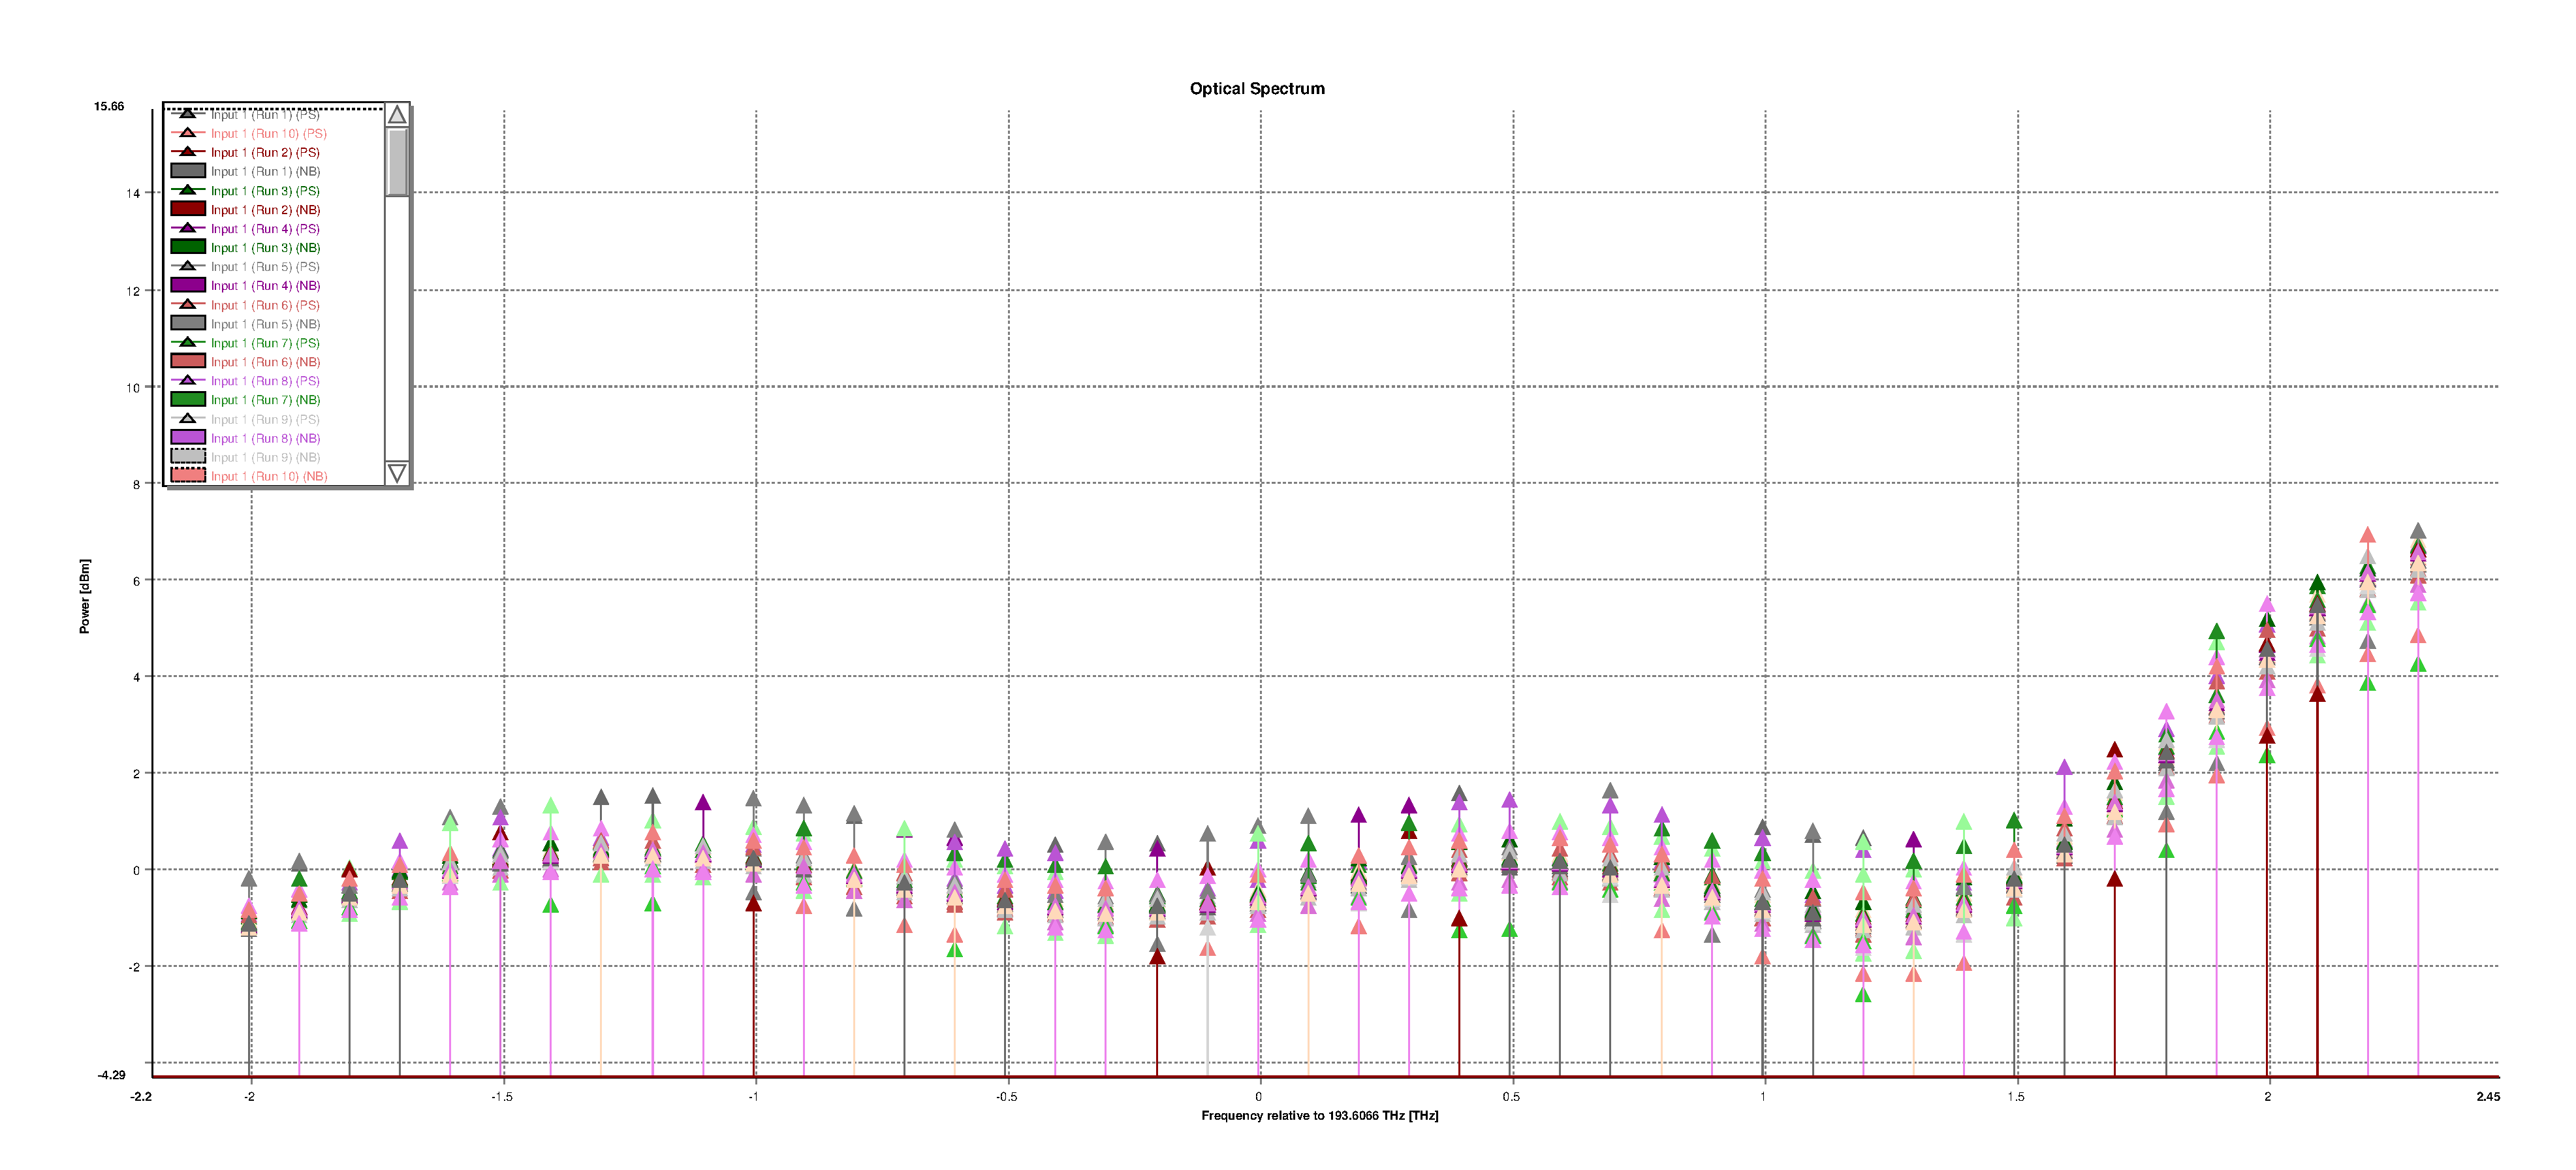
\includegraphics[width=\textwidth]{images/technical_work/section_2_data generation/sample_output_50.pdf}
        
        \label{fig:tw:vpi_50_op}
    \end{subfigure}
\end{figure}
\FloatBarrier
\subsection{Conclusion}

This section detailed the experiment designed to generated training data facilitating the development of the ML model. The training data was generated using VPI and MATLAB. The data samples are intended to emulate real-world optical signal communications that would be amplified by an EDFA operating in a backhaul network. To achieve this, the training samples were generated adhering to the ITU DWDM frequency grid using 100GHz channel spacing and 44 channels in the frequency range from 191.6THz to 195.9THz.

%say like ITU grid plan 
% and like input channel power
From the results in figure \ref{fig:tw:vpi_50_op}, the variance in the output power of each optical channel can be seen. This variability resulting from the interaction effects between optical channels is the phenomena that the ML model in section \ref{sec:ml_model} aims to predict.  


%%%%%%%%%%%%%%%%%%%%%%%%%%%%%%%%%%
% Beginning of New Section Here
%%%%%%%%%%%%%%%%%%%%%%%%%%%%%%%%%%



\section{Machine Learning Model}\label{sec:ml_model}

\subsection{Introduction}
In this section, the development of the machine learning model will be discussed. The model aims to predict the output power spectrum of an EDFA based on the input power spectrum for a given channel configuration. To this end, a fully connected neural network (NN) will be trained using data generated following the procedure outlined in section \ref{tw:sec:data_gen}. The model was developed using the Tensorflow and Keras Python libraries.

Two different model structures were trailed, and their performance was compared; 
\begin{itemize}
    \item Initially, a model with a combined network structure was implemented. This is where the input to the NN will be a vector 44 units long, each unit corresponding to the input power of a channel. The output of the network will again be a vector with the 44 output powers of each channel.

    \item Subsequently, a model with a discrete network structure was implemented. In this case, 44 different NNs were trained, each network taking the same input vector of the 44 channel powers but instead will predict the output power of a single channel. As the level of amplification varies slightly per channel, the weights of the trained network will reflect this being slightly different in each of the 44 networks.
\end{itemize}    

This chapter will be broken down into the following sections:
\begin{enumerate}
    \item Training Data
    \item Combined Network
    \item Discrete Network
    \item Model Configuration
\end{enumerate}

\subsection{Training Data}\label{subsec:ml_model:data}
\FloatBarrier
% Need to include a section about data cleaning 

% Need to include a section about using uW instead of dBM 
% Be good to include a graph of the average output power to show the variation



12,000 data samples were generated following the process discussed in section \ref{tw:sec:data_gen}. The training data was formatted, all power values were converted from $dBm$ to $\mu W$, and any noise signals were filtered from the data samples.
%should I be saying noise or ASE spontaneous noise here

\renewcommand{\arraystretch}{1.15}
\begin{table}[!h] 
    \centering
    \caption{Example training sample}
    
    \begin{tabular}[t]{l l l l l l l l }
        \textbf{Channel} & 0 & 1 & 2 & ... & 41 & 42 & 43 \\
        \hline
        \textbf{Frequency (THz)} & 191.6 & 191.7 & 191.8 & ... & 195.6 & 195.7 & 195.8 \\
        \hline
        \textbf{Input} & 1 & 0 & 1 & ... & 0 & 0 &	1 \\
        \hline
        \textbf{Output Power ($\mu W$)} & 1.370 & 0 & 1.656 & ... & 0 &	0 &	19.664 \\
        \hline
    \end{tabular}
    \label{tab:ex_data_sample}
\end{table}


As the relative input power of all channels was constant $50 \mu W$ and as the amplifier model did not account for gain saturation, the specific value of the input power was not as consequential in determining the output power spectrum. Instead, the presence or absence of a channel at a given frequency was a greater determinant. For this reason, binary values [0,1] were used to represent the presence or absence of a channel. Changing the input vectors to binary values benefited the NN, as shown in figure \ref{fig:bin_rv_ip}, allowing a lower error to be achieved during training. A typical training sample can be seen in table \ref{tab:ex_data_sample}.

\begin{figure}[h]
    \centering
    \caption{Training log for channel 19. Showing training error when input are binary or real valued. Note, graph shows epochs 10-750.   }
    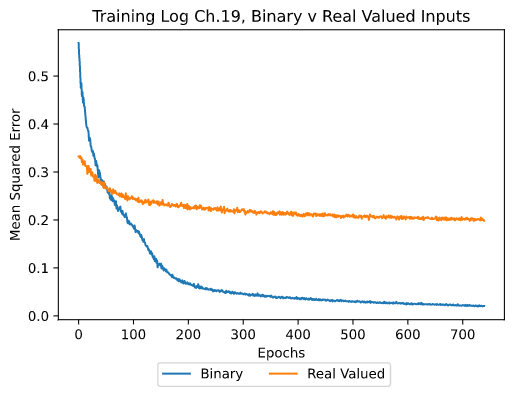
\includegraphics[width=0.66\textwidth]{project/img/ml_model/real_valued_binary.png}
    \label{fig:bin_rv_ip}
\end{figure}

When training the model a training/validation split of 80/20 was used. A different testing data set of 400 samples was generated for each channel. 

\FloatBarrier
\subsection{Combined Model} \label{sub:sec:comb_mod}
% need to mention where this model can be found, like in what notebook or whatever

\subsubsection{Development}

% Need to insert graph of the model
% Or maybe add in a table like the model summary from keras

An ML model with 44 input features, four hidden layers with 1056, 1056, 1056 and 528 neurons, respectively and an output layer of 44 units was created. The activation functions of the layers alternated between rectified linear (ReLu) and linear activation.  Dropout of 0.45 was applied after each hidden layers.


%Can make table look nicer, add a layer number col and have the words on top of each other on the first row
\begin{table}[h]
    \centering
    \caption{Combined Model Structure}
    \begin{tabular}{l l l l l l }
        \textbf{Layer} & \textbf{Type} & \textbf{Shape} & \textbf{Parameters} & \textbf{Activation} & \textbf{Dropout Rate} \\
        \hline
        0 & Input & 44 & - & - & - \\
        \hline
        \multirow[t]{2}{*}{1} & Dense & 1,056 & 47,520 & ReLu  & - \\ \cline{2-6}
        
        & Dropout & 1,056 & - & - & 45\% \\
        \hline
        \multirow[t]{2}{*}{2} & Dense & 1,056 & 1,116,192 & Linear  & - \\  \cline{2-6}
        
        & Dropout & 1,056 & - & - & 45\% \\
        \hline
        \multirow[t]{2}{*}{3} &  Dense & 1,056 & 1,116,192 & ReLu  & - \\ \cline{2-6}
        
        & Dropout & 1,056 & - & - & 45\% \\
        \hline
        \multirow[t]{2}{*}{4} & Dense & 528 & 558,096 & Linear  & - \\ \cline{2-6}
        
        & Dropout & 528 & - & - & 45\% \\
        \hline
        5 &Output & 44 & 23,276 & ReLu & - \\
        \hline
    \end{tabular}
    \label{tab:combined_model_struct}
\end{table}

The model was trained using mini-batch gradient descent and the Nadam optimiser to minimise the mean squared error (MSE). A batch size of 512 and a learning rate of $4e^{-5}$ was used.

\subsubsection{Results}
\FloatBarrier

%Need to evaluate what the R-squared metric will mean

The results of training the model for 950 epochs can be seen in figure \ref{fig:ml_model:nn_training}. After 950 epochs the training MSE loss was $= 0.2898\mu W^2$ and the validation MSE loss was $= 0.0556\mu W^2$. When evaluating the model on the test set, the test loss MSE was $= 0.0487\mu W^2$. 

\begin{figure}
     \centering
     \caption{Neural Network Training Log}
     \begin{subfigure}[b]{\textwidth}
         \centering
         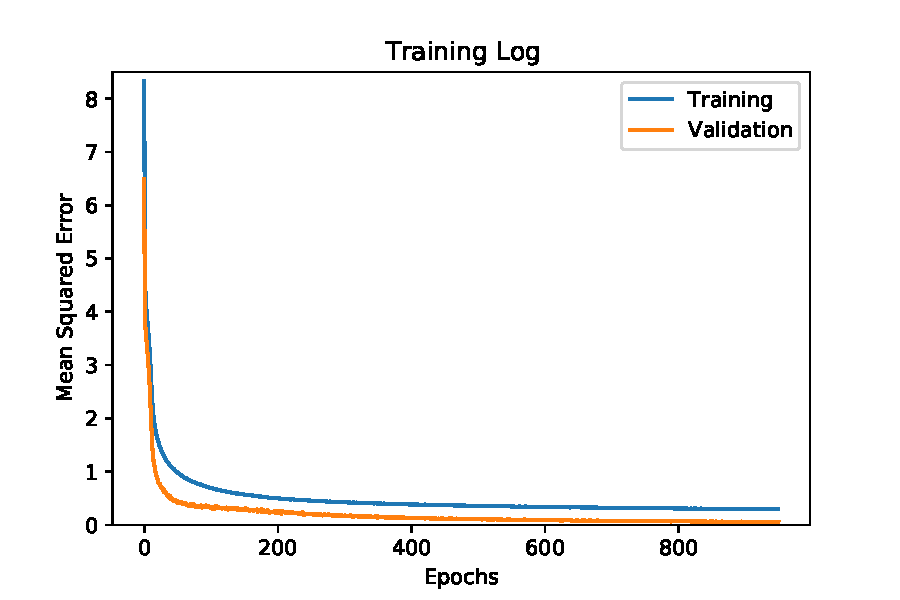
\includegraphics[width=\textwidth]{project/img/ml_model/combined/combined_training_log.pdf}
     \end{subfigure}
     \begin{subfigure}[b]{\textwidth}
         \centering
         \caption{Epochs 100 to 950.}
         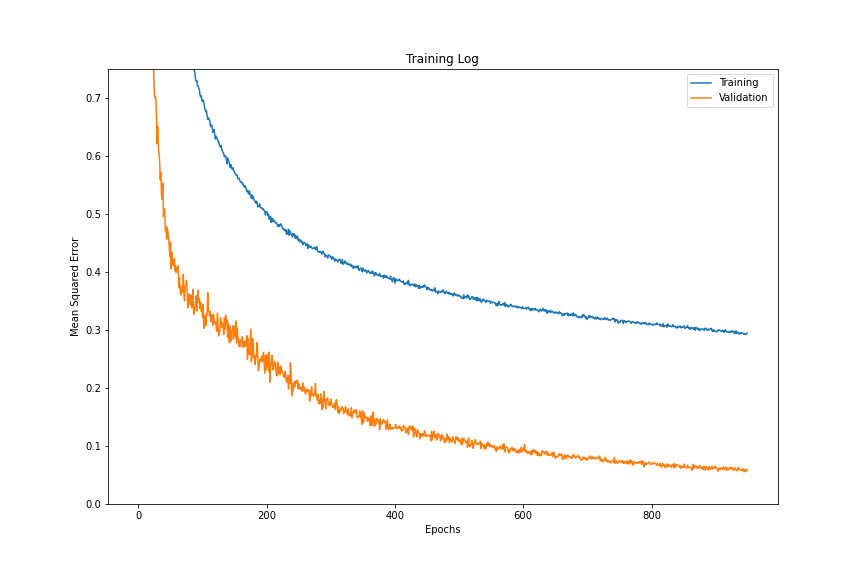
\includegraphics[width=\textwidth]{project/img/ml_model/combined/combined_training_log_inset.png}
         
     \end{subfigure}
        \label{fig:ml_model:nn_training}
\end{figure}





The test loss value is calculated as the MSE between the predicted and actual output vectors, equivalent to taking the average of the MSE over all output channels. Due to the disparity between the output powers of the lower and higher frequency channels, the MSE metric under-represents the error on the lower frequency channels. This can be seen in figure \ref{fig:ml_model:pct_err_freq} where the percentage error is graphed against the channel frequency.

A solution to this could be to use the percentage error as the loss metric. However, this option is also problematic. Any training sample where the input power of a  given channel is $0 \mu W$, the channel's output power will also be $0\mu W$. In this case, any small error in absolute terms between the predicted and true value of the output will result in a substantial percentage error.

\begin{figure}[!h]
    \centering
    \caption{Test Set percentage Error varying from Channel 1 (191.9 Thz) to Channel 43 (195.7 THz)}
    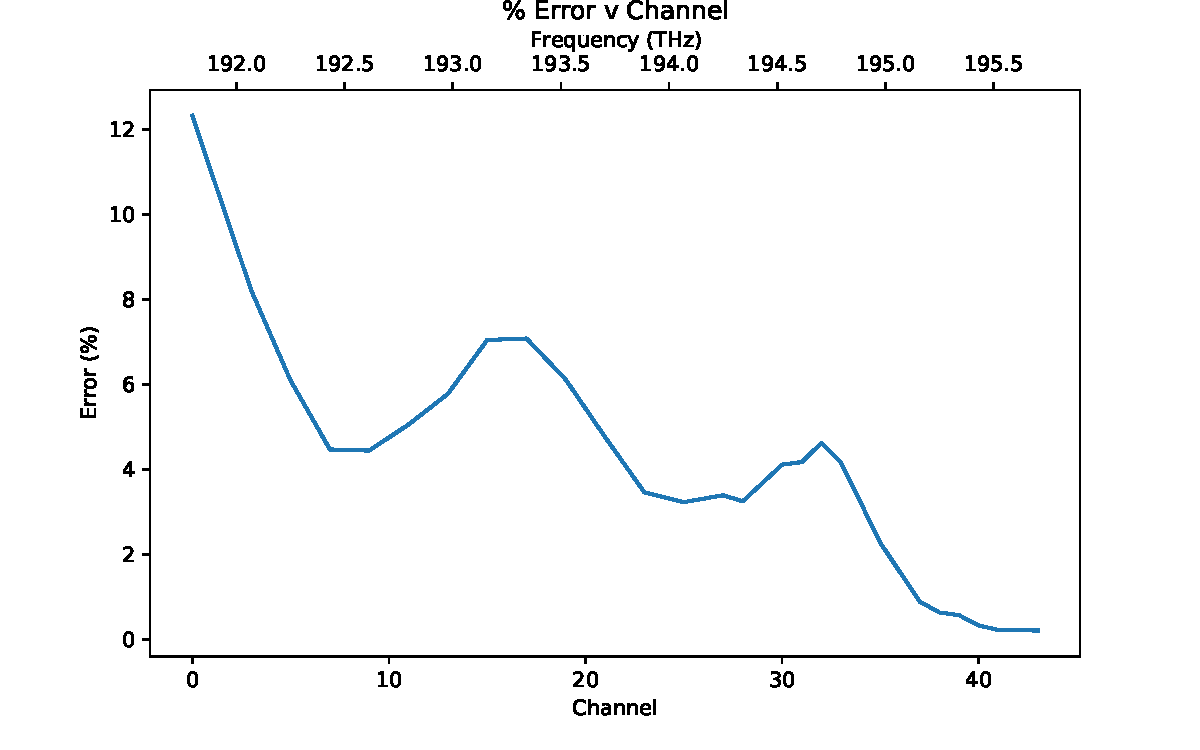
\includegraphics[width = \textwidth]{project/img/ml_model/combined/pct_err_freq.pdf}
    \label{fig:ml_model:pct_err_freq}
\end{figure}

The loss metric should be robust to training samples with $0\mu W$ values while also allowing for the uniform minimisation of errors for all channels. 



\FloatBarrier
\subsection{Discrete Model} \label{sub:sec:disc_mod}
% need to mention where this model can be found, like in what notebook or whatever

This model is comprised of 44 distinct NNs where each network will predict the output power of a single channel. The MSE will be used as the loss function for each network. It is robust to errors in training samples where the true output value is $0\mu W$, and due to the output being a single neuron, specific to a channel the relative difference between MSE values will no longer be an issue.


\subsubsection{Data}
The same training data set from section \ref{subsec:ml_model:data} was used. However, the NNs output layer is no longer a vector of 44 output channel but a single channel power. The training data was modified depending on which NN was being trained to reflect this change. Each training sample now consists of the same input vector 44 units long but a single output power value. 

The training dataset was modified specifically for the training of each of the 44 NNs. Training samples where the channel’s output power channel is $0\mu W$ are filtered out of the dataset, except for the first 500 samples. 

Each of the NNs aims to predict the impact of different channel loading conditions on the output power of a given channel; these effects only occur when the channel is active (i.e. has a non-zero output power). Therefore several thousand additional training samples where the channel’s output power is $0\mu W$ will not benefit the training process. The first 500 samples were not filtered to ensure there will be some training samples where the output power is $0\mu W$.
%Could add a bit about the average split between the amount of samples where a given channel was on for and when it wasn't 



\subsubsection{Development}


Each NN comprises seven fully connected layers; one input layer with five hidden layers and one output layer. The input layer consists of 44 neurons, the hidden layers consist of 360, 180, 180, 90 and 45 neurons, respectively, and the output layer is a single neuron. Dropout of 45\% is applied after the first four hidden layers and 20\% after the fifth. 


%Can make table look nicer, add a layer number col and have the words on top of each other on the first row
\begin{table}[!h]
    \centering
    \caption{Discrete Model Structure}
    \begin{tabular}[b]{l l l l l l }
        \textbf{Layer} & \textbf{Type} & \textbf{Shape} & \textbf{Parameters} & \textbf{Activation} & \textbf{Dropout Rate} \\
        \hline
        0 & Input & 44 & - & - & - \\
        \hline
        \multirow[t]{2}{*}{1} & Dense & 360 & 16,200 & ReLu  & - \\ \cline{2-6}
        
                & Dropout & 360 & - & - & 45\% \\
        \hline
        \multirow[t]{2}{*}{2} & Dense & 180 & 64,980 & Linear  & - \\ \cline{2-6}
        
        & Dropout & 180 & - & - & 45\% \\
        \hline
        \multirow[t]{2}{*}{3} & Dense & 180 & 32,580 & ReLu  & - \\ \cline{2-6}
        
        & Dropout & 180 & - & - & 45\% \\
        \hline
        \multirow[t]{2}{*}{4} & Dense & 90 & 16,290 & Linear  & - \\ \cline{2-6}
        
        & Dropout & 90 & - & - & 45\% \\
        \hline
        \multirow[t]{2}{*}{5} & Dense & 45 & 4,095 & ReLu  & - \\ \cline{2-6}
        
        & Dropout & 45 & - & - & 20\% \\
        \hline
        6 & Output & 1 & 46 & ReLu & - \\
        \hline
    \end{tabular}
    \label{tab:discrete_model_struct}
\end{table}

Each network was trained using mini-batch gradient descent, and the Nadam optimiser, a batch size of 512 and a learning rate of $1e^{-4}$ was used.


\FloatBarrier
\subsubsection{Results}
 
The training log for channel 19 is shown in figure \ref{fig:ml_model:disc_train_log}; this graph is representative of the training of any of the NNs. The training and validation mean percentage error (MPE) for each NNs after training for 750 epochs can be seen in figure \ref{fig:ml_model:disc_train_val}. The per-channel MPE is significantly lower using the discrete model structure than the combined model structure, as shown in figure \ref{fig:ml_model:pct_err_freq}.

\begin{figure}
     \centering
     \caption{Training log for channel 19, showing training and validation loss.}
     \begin{subfigure}[b]{\textwidth}
         \centering
         \caption{Full log.}
         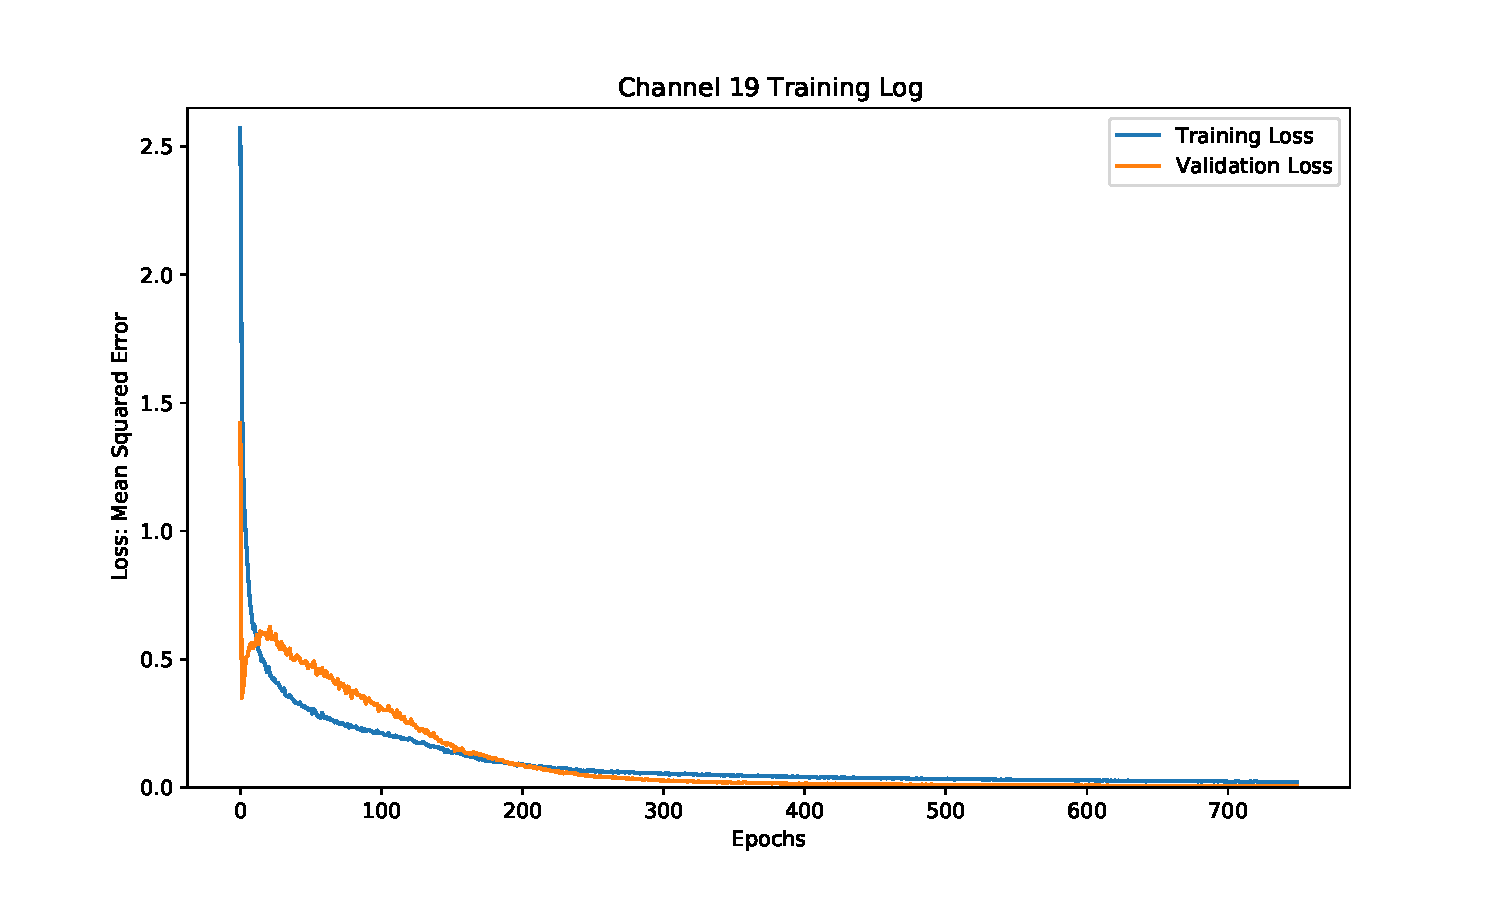
\includegraphics[width=\textwidth]{project/img/ml_model/discrete/Channel 19 Training Log.pdf}
     \end{subfigure}
     \vspace{-4em}
     \begin{subfigure}[b]{\textwidth}
         \centering
         \caption{Epochs 100 to 750.}
         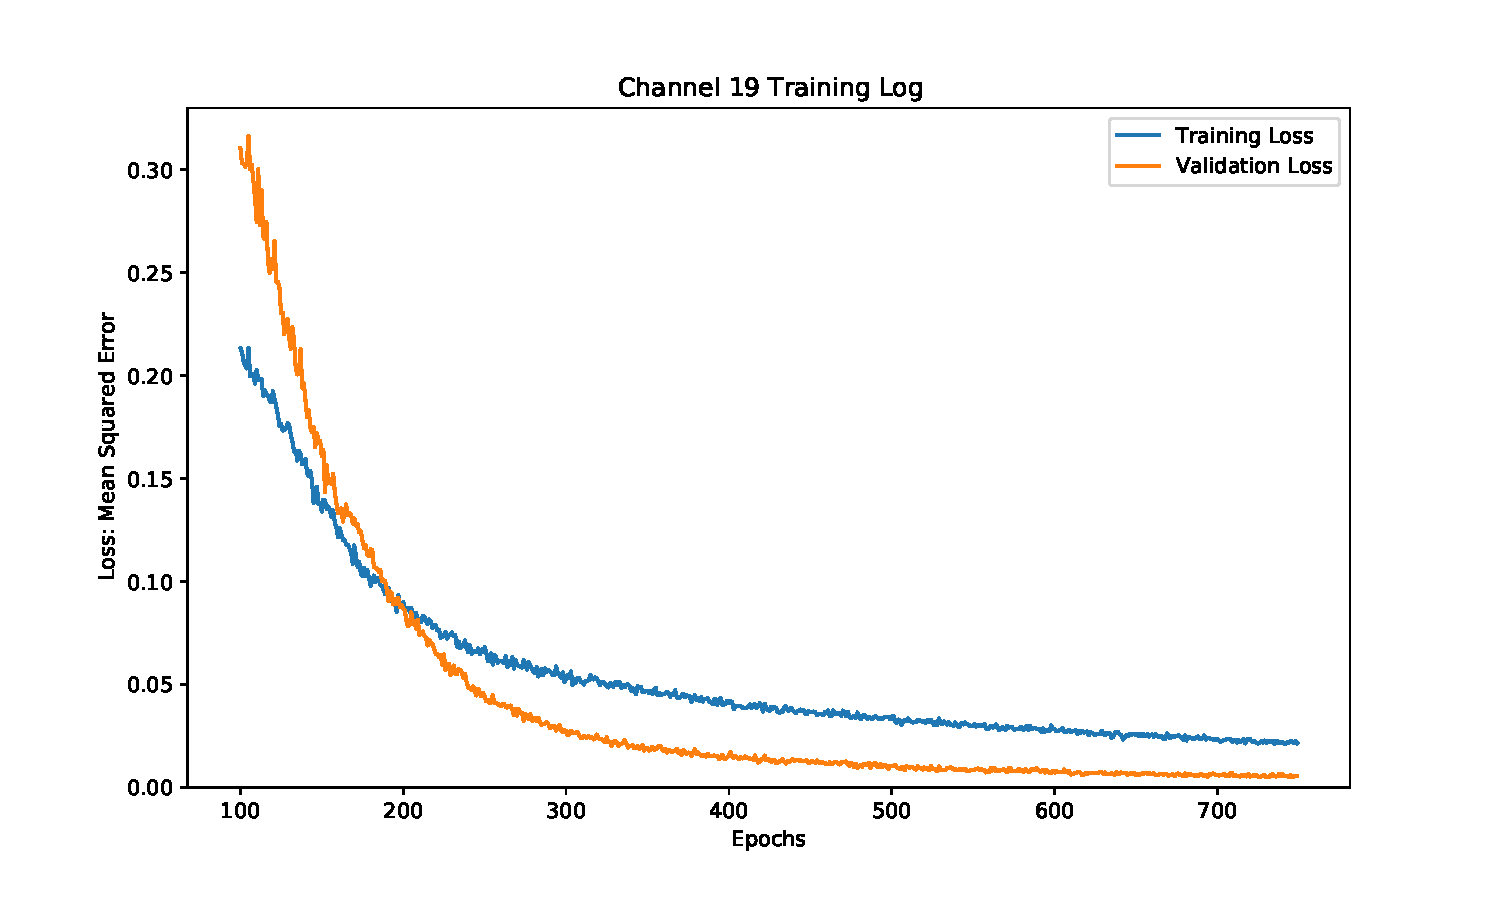
\includegraphics[width=\textwidth]{project/img/ml_model/discrete/Channel 19 Training Loginset.pdf}
     \end{subfigure}
        \label{fig:ml_model:disc_train_log}
\end{figure}

% Include a picture of a training graph for the model

\begin{figure}
    \centering
    \caption{MPE of each Neural Network after training for 750 epochs. The standard deviation is the measure of variability.}
    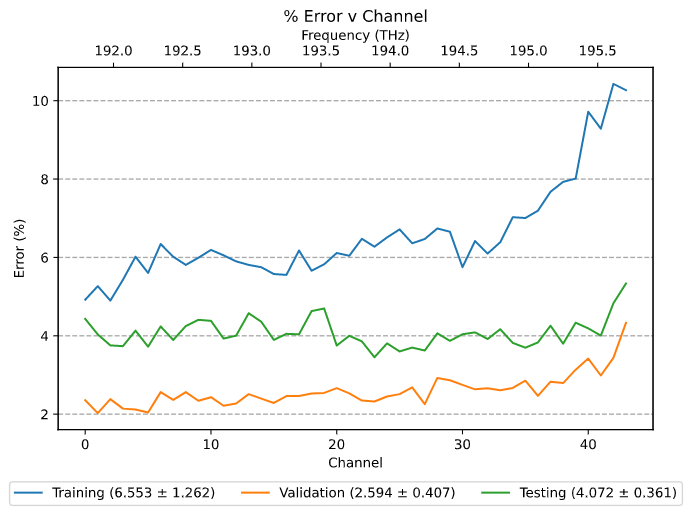
\includegraphics[width=\textwidth]{project/img/ml_model/discrete/percent_error.png}
    \label{fig:ml_model:disc_train_val}
\end{figure}

\FloatBarrier
\subsection{Model Configuration}

\FloatBarrier
\subsubsection{Optimiser} \label{subsec:optimiser}

\begin{figure}[h]
    \centering
    \caption{Convergence of Nadam optimiser v Stochastic Gradient Decent, training log for channel 19}
    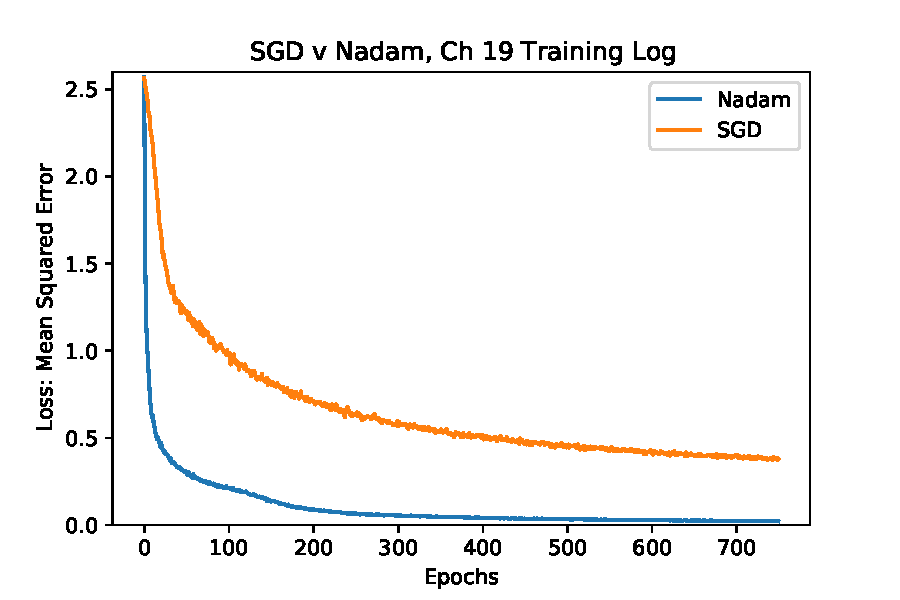
\includegraphics[width=\textwidth]{project/img/ml_model/discrete/SGD v Nadam, Ch 19 Training Log.pdf}
    \label{fig:ml_model:sgd_nadam}
\end{figure}

The Nadam optimiser was used for the gradient descent optimisation of the NN. The choice of optimiser resulted from experimentation, training sample models, and measuring the performance of various gradient decent optimisers.

As can be seen in figure \ref{fig:ml_model:sgd_nadam} the Nadam optimiser leads to convergence much earlier during training than with stochastic gradient descent, which has not converged even after 750 training epochs.


The Nadam optimiser is a combination of the Nesterov Accelerated Gradient and Adam optimiser. The Adam optimiser is modified to include Nesterov momentum by replacing the momentum vector of the previous time step $\hat{m}_{t-1}$ with that of the current momentum vector $\hat{m}_t$ when updating the weights, in equation \ref{eq:ml_model:nadam_main}.

As with the Adam optimiser, the momentum term $\hat{m}_t$ (equation \ref{eq:ml_model:nadam_momentum}) is the exponential weighted average of gradients. The learning rate $\alpha$ is decayed by $\hat{v}_t$ (equation \ref{eq:ml_model:decay_lr}), the square of the exponential moving average of previous gradients. $ [\frac{\delta L}{\delta w_t}]$ is the gradient and $\epsilon$ is a small positive constant to avoid division by 0.The optimiser can be tuned using $\alpha$, $\beta_1$ and $\beta_2$ parameters, these correspond to the leaning rate, the decay rate of the gradient and the decay rate of the square of the gradients. The following values were used; $\alpha = 1e^{-4}$, $\beta_1 = 0.9$, $\beta_2 = 0.99$.
%Need to add in a refrence to Nadam paper here
% Dozat, T. (2016). Incorporating Nesterov Momentum into Adam. ICLR Workshop, (1), 2013–2016. 







%\begin{equation}
\begin{gather}
    w_{t+1} = w_t - \big( \frac{\alpha}{\sqrt{\hat{v_t} + \epsilon}} \big) \Bigg( \beta_{1} \hat{m_{t}} + \frac{(1 - \beta_1)}{(1 - \beta^{t}_1)} \bigg[\frac{\delta L}{\delta w_t}\bigg] \Bigg) \label{eq:ml_model:nadam_main} \\ 
    \hat{m_t} = \frac{1}{1 - \beta^{t}_1} \times \Bigg( \beta_{1} \hat{m}_{t-1} + (1 - \beta_1) \bigg[\frac{\delta L}{\delta w_t}\bigg] \Bigg) \label{eq:ml_model:nadam_momentum} \\
    \hat{v_t} = \frac{1}{1 - \beta^{t}_2} \times \Bigg( \beta_2 \hat{v}_{t-1} + ( 1- \beta_2) \bigg[\frac{\delta L}{\delta w_t}\bigg]^2 \Bigg) \label{eq:ml_model:decay_lr}
\end{gather}
%\end{equation}





\subsubsection{Loss Function} \label{subsec:loss_func} \FloatBarrier


\begin{figure}[h]
    \centering
    \caption{Comparison of Mean Squared Error v Mean Absolute Percentage Error (MAPE) loss functions. Note the second y axis for MAPE, is scaled by $1e^7$.}
    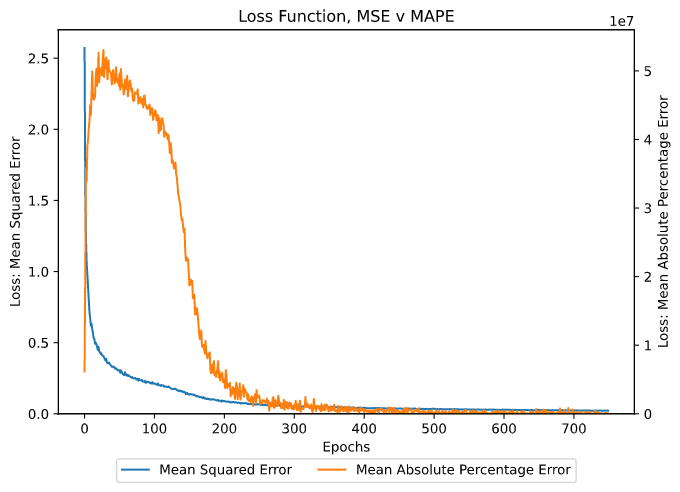
\includegraphics[width=\textwidth]{project/img/ml_model/discrete/mse_mpe.png}
    \label{fig:ml_model:mse_mpe}
\end{figure}

The choice of loss function impacts the training of the NN. The NNs are being trained to solve a regression problem; thus, the MSE and Mean Absolute Percentage Error (MAPE) were considered for the loss function. The MSE loss and MAPE loss can be seen in the training log in figure \ref{fig:ml_model:mse_mpe}. To note is the relative noisiness of the MAPE and the large range of values that the loss function takes, from $\sim 5e^7\%$ to $0\%$.

MAPE is extremely sensitive to errors when the true value is very small relative to the predicted value, particularly in this training dataset when the true value is $0\mu W$. The large range over which MAPE varies results from errors when the true value of a training sample is $0 \mu W$. The large noise of the MAPE is a scaling of the noise in the MSE plot, scaled due to the error being calculated on a relative basis.

This over-sensitivity towards 0 values is an undesirable property of MAPE. The model aims to predict the impact of channel interaction effects on the output of a given channel. These effects are only present when the output of the channel is nonzero. Due to these factors, MSE was used as the loss function. 



\FloatBarrier


\subsection{Conclusion}

This section has provided an overview of a machine learning model's development through a series of experimental tests used to determine the ideal model structure, data representation, and loss metrics for the model.

Resulting from these tests is a model consisting of 44 separate NNs, each trained to predict the output of a single optical channel. Each network was comprised of 5 hidden layers using linear and ReLu activation. Training occurred on a data set of 12,000 samples using the Nadam optimiser, with a learning rate of $1e^{-4}$ and mini-batch gradient descent with a batch size of 512. MSE was used as the loss function. The trained model has an average per channel error of $4.07\%$. 
 